\documentclass[a4paper, 10pt]{article}

\usepackage{rotating}

\usepackage{graphicx}
\usepackage[caption=false,font=small]{subfig}

\usepackage{hyperref}

\usepackage{mma} % Mathematica

\usepackage{booktabs}
\usepackage{threeparttable} % For table with footnotes

% fun with danger signs
%\usepackage{stackengine}
%\usepackage{scalerel}
%\usepackage{xcolor}
%\newcommand\dangersign[1][2ex]{%
%  \renewcommand\stacktype{L}%
%  \scaleto{\stackon[1.3pt]{\color{red}$\triangle$}{\tiny\bfseries !}}{#1}%
%}

% make straight double quotes with \mathtt{"} in math mode
\DeclareMathSymbol{"}{\mathalpha}{letters}{`"}

\title{IBM ExaBounds manual}
\author{R. Jongerius\\IBM Research, The Netherlands}
\date{\today}

\begin{document}

\maketitle
\section*{Abstract}

This manual describes how to use IBM ExaBounds for performance and power modeling. ExaBounds is implemented in Mathematica and requires a Mathematica license to be used. There is a GUI available to use IBM ExaBounds, but it is also possible to use the Mathematica language to create scripts for automation of design-space exploration experiments. The current GUI can be used for the processor performance models. For the network performance models, IBM ExaBounds provides the user with an
API that can be used to create Mathematica scripts.


\tableofcontents

\section{Introduction}

This document describes how to use IBM ExaBounds, which implements the performance model described in~\cite{Jongerius2016}. Section~\ref{sec:100:setup} describes how to set up the environment correctly. Section~\ref{sec:200:gui} discusses how to use the graphical user interface of IBM ExaBounds. Section~\ref{sec:300:notebook} describes how to use the API of the notebook to create your own automated design-space exploration notebooks.


\section{Setup}
\label{sec:100:setup}

IBM ExaBounds consists of an executable notebook (ExaBoundsLite.nb) and a large set of supporting packages. It can only be executed with the full version of Wolfram Mathematica (version 11.2 and later).

\subsection{McPAT}

In order to predict the power consumption of compute nodes, McPAT~\cite{Li2009} has to be available on the system. McPAT is used to predict power consumption of the processor cores and caches. ExaBounds expects the McPAT executable named \textsc{mcpat} (or \textsc{mcpat.exe} for Windows) to be available in a directory listed in the \textsc{\$PATH} environment variable. ExaBounds is tested with McPAT 1.0, it can be downloaded from \url{http://www.hpl.hp.com/research/mcpat/}.

\subsection{CACTI}

The power consumption of the main memory can be predicted using either the build-in power model IBM Memory-Scheduler-Agnostic Power Model~\cite{Poddar2017} or CACTI~\cite{Thoziyoor2008}. In case CACTI is desired, it needs to be available via the \textsc{\$PATH} environment variable as well. ExaBounds only works with CACTI 5.3, which can be downloaded from \url{http://www.hpl.hp.com/research/cacti/}. The executable name has to be \textsc{cacti53} (or \textsc{cacti53.exe} for Windows).

The memory power model can be selected in the CDF or notebook and is default set to IBM Memory-Scheduler-Agnostic Power Model.

\section{Workflows}
\label{150:sec:workflows}

ExaBounds is part of a larger set of tools that together can be used for performance and power analysis of future (exascale) computing systems. The set of tools encompasses IBM Platform-Independent Software Analysis~\cite{Anghel2016} for hardware-independent application profiling. The generates profiles serve as input for the workload extrapolation models of IBM Exascale Extrapolator~\cite{Mariani2016} or directly to IBM ExaBounds.

Figure~\ref{fig:150:workflow} shows the potential workflows of our tooling. The lower part of the figure shows the most basic workflow: IBM Platform-Independent Software Analysis is used to profile a single run of an application. The generated profile (in JSON format) is loaded in IBM ExaBounds and predictions are made for an architecture of for a set of architectures (design-space exploration).

\begin{figure}
 \centering
 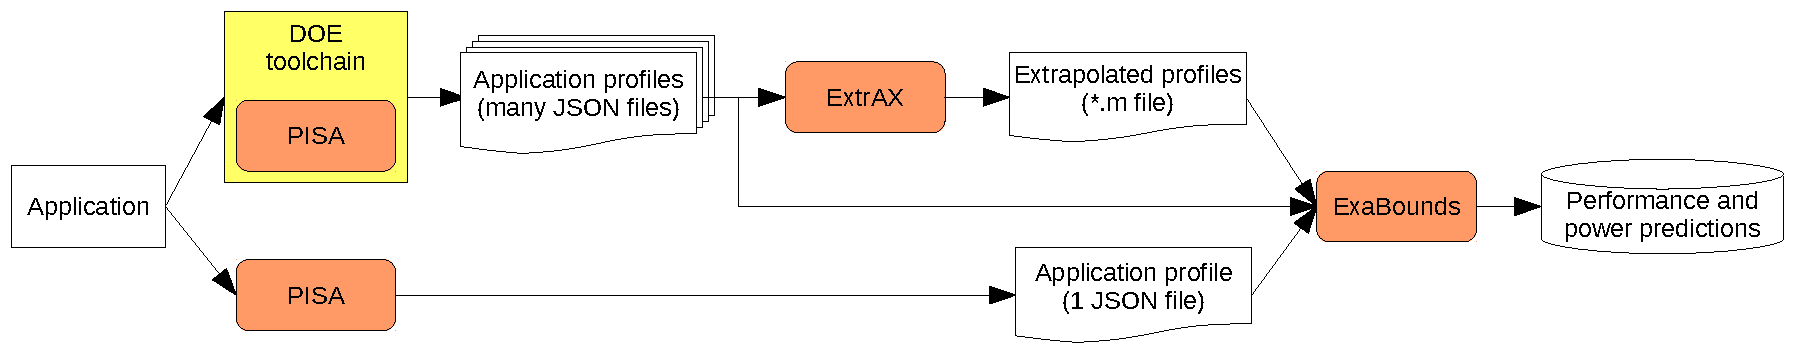
\includegraphics[width=\columnwidth]{img/workflow.pdf}
 \caption{Different workflows of our tool flow. IBM Platform-Independent Software Analysis is used to extract profiles of applications. Such profiles can be extrapolated to exascale using IBM Exascale Extrapolator. ExaBounds predicts the performance and power consumption of the application running on different architectures.}
 \label{fig:150:workflow}
\end{figure}

The top part of the figure shows a more complex workflow. Applications can behave differently for different workloads (both workload size or data content), or, for parallel applications, threads within an application may behave differently for different amounts of exploited parallelism. To capture this dynamism, a design of experiments (DOE) can be performed to sample the behavior of the application at different operating points. This will involve multiple runs of the profiler and will result in a set of JSON output files. These output files can subsequently be directly used in ExaBounds for performance and power predictions, but it is also possible to first use IBM Exascale Extrapolator to extrapolate the workload profiles to a point that isn't sampled (using machine learning). As an example, the application profiles can be exploited to an exascale-sized workload, a workload size that cannot be analyzed by IBM Platform-Independent Software Analysis directly due to constraints on the system which is used for profiling. IBM Exascale Extrapolator generates a Mathematica file containing the profiles of the application at the targed (scaled) operating points. This Mathematica file can be similarly read by IBM ExaBounds for predictions.

\section{Default architectures and algorithms}

\begin{minipage}[t]{0.05\textwidth}
~\\
\Huge !
\end{minipage}
\begin{minipage}[t]{0.94\textwidth}
IBM ExaBounds ships with a set of default loaded architectures and algorithms. The architectural properties aim to reflect their respective architectures as good as possible. Most properties are retrieved from public sources on the Internet. Some of the remaining properties cannot be found and are based on reasonable estimates. It is advised to carefully check default architectures and algorithms for correctness for real experiments.\end{minipage}
~\linebreak

\section{Graphical user intefrace}
\label{sec:200:gui}

The following section describes the usage of the IBM ExaBounds graphical user interface.

\subsection{Loading application profiles}

IBM ExaBounds can load application profiles in the JSON format generated by IBM Platform-Independent Software Analysis~\cite{Anghel2016} or in the Mathematica format generated by IBM Exascale Extrapolator~\cite{Mariani2016}. This can be used to use ExaBounds to analyze any application that can be analyzed using IBM Platform-Independent Software Analysis. Figure~\ref{fig:200:loadjson} shows the GUI element that can be used to load algorithms. It shows the algorithms already loaded. The \textsc{default} algorithm is loaded by default and contains two profiles of the Graph 500~\cite{Graph500} benchmark set. By clicking \textsc{Import JSON file} a dialog box opens to load new IBM Platform-Independent Software Analysis files in JSON format. Similarly, clicking \textsc{Import mathematica file} allows loading an IBM Exascale Extrapolator file in Mathematica format *.m (by default, IBM Exascale Extrapolator stores data in the \textsc{predictedAlgorithm} symbol).

\begin{figure}
  \centering
  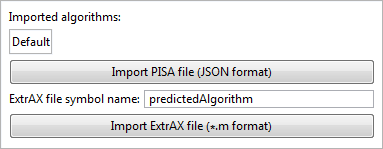
\includegraphics[width=0.6\columnwidth]{img/load-json.png}
  \caption{Import algorithms GUI element.}
  \label{fig:200:loadjson}
\end{figure}

During loading of an input file, several warning messages can be displayed at the bottom of the CDF file. Two types of warning messages can exist: missing properties and invalid data. In case of invalid data, there is a problem with the data in the input file. For example, the summation of all instruction fractions does not add up to 1. % The PISA file or ExtrAX extrapolation models should be inspected and potentially be regenerated.

An example missing properties warning is:
\begin{mma}
	\Warning{AlgorithmFromFileJSON`LoadAlgorithmJSON::missingproperties} The properties \linebreak \{externalLibraryCallCount, instrReuseDistribution, memoryFootprint, mpiCommunicationVector, mpiDataExchanged, mpiInstructionMix, openMPinstructionMix\} were not read correctly for the file: file.out. \\
\end{mma}
The warning states that several properties are missing in the profile file and therefor not loaded. Care should be taken that all properties that are relevant for a specific analysis are loaded for valid performance and power analysis results. Table~\ref{tbl:200:properties} list the common properties\footnote{These properties usually cover several parameters in the profile files.} and for which parts of the models they are used. Note that all properties related to core modeling should always be loaded.

\begin{table}
  \centering
  \small
  \caption{Properties and their use in the analytic models.}
  \label{tbl:200:properties}
  \begin{threeparttable}
    \begin{tabular}{lll}
    	\toprule
      \textbf{Property} & \textbf{Use} & \textbf{Always needed?} \\
      \midrule
      instructionMix & Core modeling & Yes \\
      dataReuseDistribution\tnote{1} & Core modeling & Yes \\
      instrReuseDistribution & Not used & No \\
      memoryFootprint & Not used & No \\
      branchEntropy & Not used & No \\
      bestMisprectionRate & Core modeling & No \\
      ilp & Core modeling & Yes \\
      ilptype & Core modeling & Yes \\
      inorder ilp\tnote{2} & In-order core modeling & No \\
      inorder ilptype\tnote{2} & In-order core modeling & No \\
      registerAccesses & Core modeling & Yes \\
      openMPinstructionMix & Not used & No \\
      mpiInstructionMix & Not used & No \\
      mpiDataExchanged & Not used & No \\
      mpiCommunicationVector & Not used & No \\
      externalLibraryCallCount & Not used & No \\
      processId & Not used & No \\
      threadId & Not used & No \\
      \bottomrule
    \end{tabular}
    \begin{tablenotes}
      \item[1] The data reuse distribution for two cache line sizes (64 and 128) is being read, only one is needed. However, a warning will be generated when only one is available.
      \item[2] Will be deprecated. In-order modeling will be done using the regular ILP parameters.
    \end{tablenotes}
  \end{threeparttable}
\end{table}

\subsection{Loading architectures}

Architectures are also described using JSON files. In total, three different types of JSON files can be loaded: processor architecture files, memory architecture files and network architecture files. Each file contains a set of parameters that describe an architecture, the parameters are described in Appendix~\ref{app:architecture-parameters}. During execution of the models, an processor, memory, and network architecture are combined to describe a complete system.

IBM ExaBounds loads a set of default architectures that can be used. Custom architectures can be loaded using the architecture interface as shown in Figure~\ref{fig:200:loadarchitectures}.

\begin{figure}
  \centering
  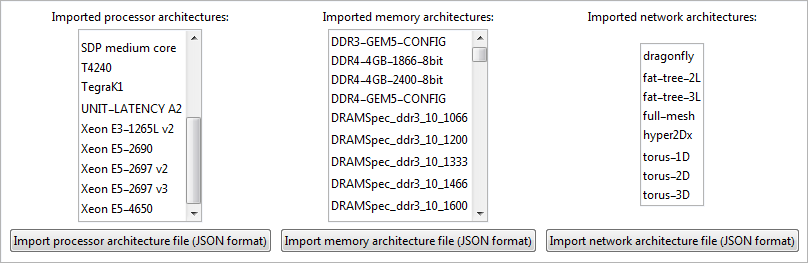
\includegraphics[width=0.95\columnwidth]{img/load-architecture.png}
  \caption{Import architectures GUI element.}
  \label{fig:200:loadarchitectures}
\end{figure}

\subsection{Performing a basic performance and power analysis for a single thread single-node}

\subsubsection{Choosing the architecture}

The first step to do a basic performance and power analysis is to select the architecture to study.
Figure~\ref{fig:200:architecturepicker} shows the architecture selection box. The drop-down menu allows to select any of the predefined machine configurations. By clicking the small downward arrow, a table expands which shows the architectural parameters of the choosen configuration.

\begin{figure}
  \centering
 	\subfloat[Architecture picker]{
		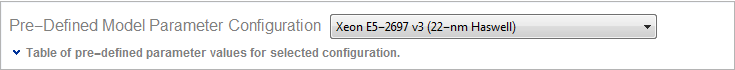
\includegraphics[width=0.98\columnwidth]{img/archpicker.png}
		\label{fig:200:architecturepicker}
	}\\
	\subfloat[Application picker]{
		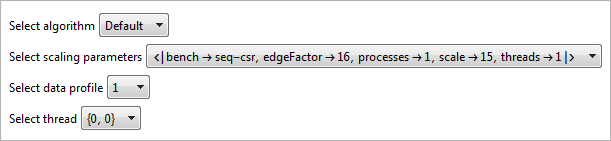
\includegraphics[width=0.8\columnwidth]{img/apppicker.png}
		\label{fig:200:applicationpicker}
	}
	\caption{Selection boxes to select an architecture and algorithm for a basic performance and power analysis.}
	\label{fig:200:architectureapplicationpicker}
\end{figure}

\subsubsection{Choosing the application}

After selection of the architecture, an application can be selected to analyze. Figure~\ref{fig:200:applicationpicker} shows the four selection boxes needed to select a thread from an application. From top to bottom, the four boxes select: the algorithm, an associated set of scaling parameters (e.g., the data size), a data profile (e.g., different runs with different data), and finally a specific thread.

\subsubsection{Results}

After selection, the results update automatically and is presented in two forms: the bottleneck plot and a table.

Figure~\ref{fig:200:bottleneckplot} shows the bottleneck plot of the selected combination of architecture and application. The plot gives insight in the architectural and application parameters that limit the performance of the thread. The blue bullets show absolute constraints, while the orange crosses show relative constraint. The relative constraints are always relative of an absolute constraint: shifting the absolute constraints will also shift the relative constraints. The absolute constraints are independent of each other. In the example, the absolute constraint limiting performance is the ILP per type mem, which indicates that the limited parallelism in the memory access or their long latency is expected to limit performance on a real system. The branch misprediction penalty decreases performance further.

\begin{figure}
  \centering
  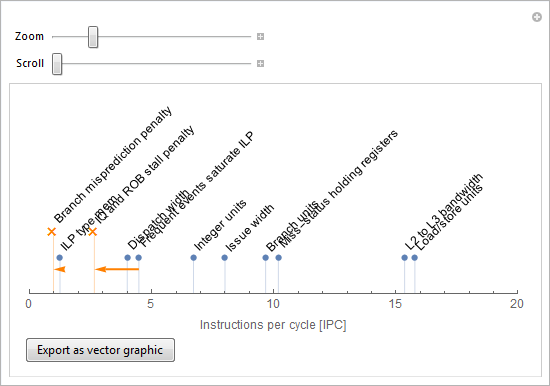
\includegraphics[width=0.7\columnwidth]{img/bottleneckplot.png}
  \caption{Bottleneck plot for the selected architecture and application pair.}
  \label{fig:200:bottleneckplot}
\end{figure}

The results in table-form are shown in Figure~\ref{fig:200:resultstable}. By default, the power analysis using McPAT, and IBM Memory-Scheduler-Agnostic Power Model or CACTI is disabled. By checking the checkbox, the power analysis can be enabled and will run automatically. Please note that this can take some time to finish during which it may appear that the system hangs.

\begin{figure}
  \centering
  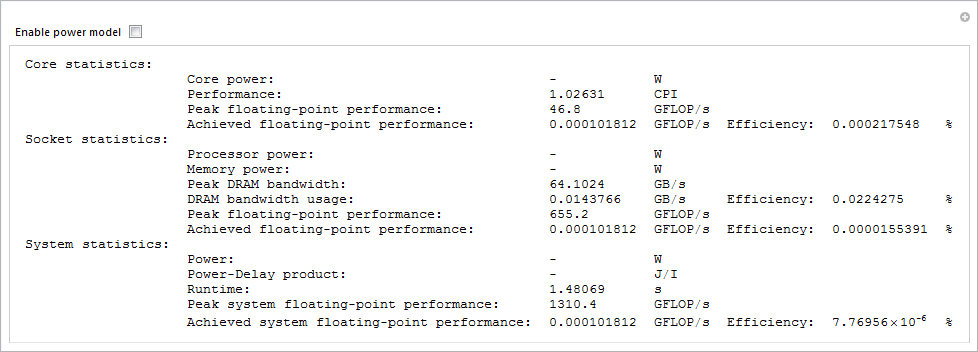
\includegraphics[width=0.9\columnwidth]{img/resultstable.png}
  \caption{Results table for the selected architecture and application pair.}
  \label{fig:200:resultstable}
\end{figure}

\subsection{Multi-core analysis}

A multi-core analysis can be performed using the multi-core GUI interface as is shown in Figure~\ref{fig:200:multicore}. It is a known issue that this interface is sometimes slow to respond.

\begin{figure}
  \centering
  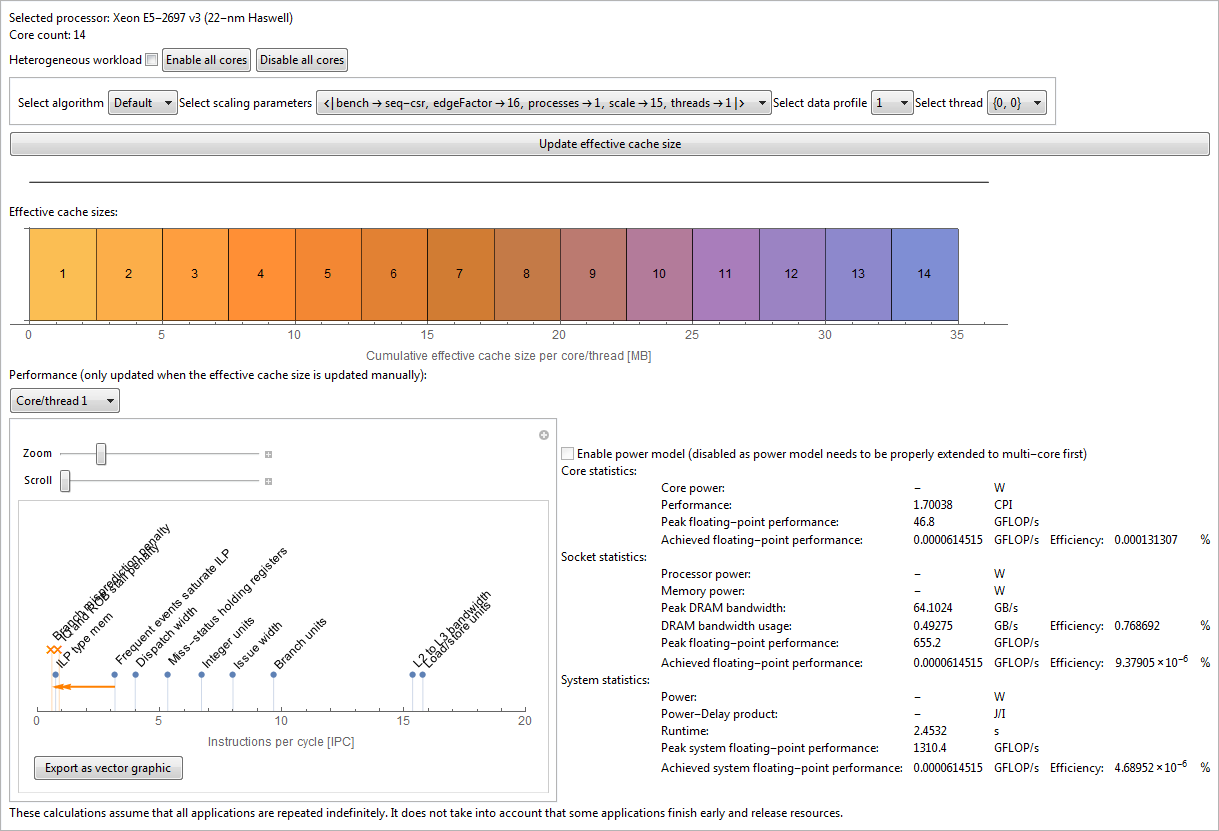
\includegraphics[width=1.0\columnwidth]{img/multicoregui.png}
  \caption{Multi-core analysis GUI and results.}
  \label{fig:200:multicore}
\end{figure}

The first step is to select an architecture with the architecture selection box as shown in Figure~\ref{fig:200:architecturepicker}. Then, the required threads can be selected to run on the target platform. The GUI gives the choice to run a homogeneous workload (all threads the same) or a heterogeneous workload (all threads different). After specifying the right threads, click the ``Update results'' button to recalculate the effective cache size for each thread and update the results. The results will be shown with a similar bottleneck plot and table as shown before.

\subsection{Design-space exploration}

T.b.d.

\subsection{Troubleshooting}

It can happen that external tools like McPAT fail or that for other reasons IBM ExaBounds returns wrong answers due to some error. Usually, re-evaluating the model does not help as IBM ExaBounds caches intermediate results to speed up evaluation. The three buttons at the bottom of the notebook can be used to clear all caches. Notice that this means that all analysis will be performed again.

\section{Programming with the IBM ExaBounds API}
\label{sec:300:notebook}

IBM ExaBounds can be used with custom notebooks by programming in Mathematica while using the IBM ExaBounds API. This section describes how to the use API.

\subsection{Starting point}

As the starting point, one should always load the \textsc{ExaBoundsLite.nb} notebook and execute it contents. This will make sure all the packages are loaded and the data structures are initialized.

\subsection{Loading algorithms}

Algorithms can be loaded automatically without using the GUI. First, create a list of IBM Platform-Independent Software Analysis profile files (full path and filename) to load:
\begin{mma}
	\In |dir| = \mathtt{"}/home/user/\mathtt{"}; \\
  \In |JSONfileList| = \{ \linebreak
    |dir| <> \mathtt{"}app1.out\mathtt{"}, \linebreak
    |dir| <> \mathtt{"}app2.out\mathtt{"}, \linebreak
    |dir| <> \mathtt{"}app3.out\mathtt{"} \linebreak
  \}; \\
\end{mma}

The profile files in the list can now be loaded using \textsc{AddAlgorithm}:
\begin{mma}
  \In |algorithmIdentifiers| = \linebreak |AddAlgorithm|[|ExaBoundsAlgInfo|, \#]~\& /@ |JSONfileList|; \\
\end{mma}

The call to \textsc{AddAlgorithm[]} for each file returns a list of \textsc{algorithmIdentifiers}, each corresponding to the first data profile and first thread in the profile files (in the same order as the files in the file list). Each of the identifiers consists of four elements identifying the application, scaling parameter, data profile, and thread. Essentially, this is in an index into the drop-down boxes in Figure~\ref{fig:200:applicationpicker}. Note that the GUI elements in the \textsc{ExaBoundsLite.nb} notebook (e.g., Figure~\ref{fig:200:loadjson}) are also updated to reflect loading of the files.

IBM Exascale Extrapolator output files can be loaded as well automatically. One can use the \textsc{Get[]} to load the file subsequently followed by a call to \textsc{AppendAlgorithmAnalysis[]} to load the data into the IBM ExaBounds data structures:
\begin{mma}
  \In |Get|[\mathtt{"}/home/user/extrax-file.m\mathtt{"}]; \\
  \In |AppendAlgorithmAnalysis|[|ExaBoundsAlgInfo|, |predictedAlgorithm|]; \\
\end{mma}
Here, \textsc{ExaBoundsAlgInfo} is the name of the IBM ExaBounds data structure and \textsc{predictedAlgorithm} is the default name of the symbol defined in the IBM Exascale Extrapolator output file which contains the extrapolated application profiles.

For the network performance models, the user is required to set the communication pattern of the application. The pattern needs to be defined per process profile (if the profile is extracted from a IBM Platform-Independent Software Analysis) or per class (cluster) profile (if the profile is extracted from an extrapolated IBM Exascale Extrapolator file), even though the pattern is the same pattern for all processes or classes (clusters) of processes. If the communication pattern is not known a-priori, the user should manually examine the communication matrix that shows how much data the processes exchange among each other during the execution of the program. Currently IBM ExaBounds supports three types of HPC patterns: \textit{uniform} (uniform all-to-all), \textit{shift} (with shift value \textit{value}) and \textit{nne2D} (2-dimension nearest-neighbor with an application domain size of D1$\cdot$D2). The user can set the communication pattern as follows:

\begin{mma}
	\In |swProfile| = |ExaBoundsAlgInfo[algName][scalingConfiguration]| \linebreak |[[dataProfile]][{processId, 0}]|; \\
	\In |swProfile| = |SetKeyValue[swProfile|, \mathtt{"}|CommunicationPattern|\mathtt{"}, \linebreak
	<\mathtt{\mid"}|type|\mathtt{"} \rightarrow  \mathtt{"}|nne2D|\mathtt{"},  \mathtt{"}D1\mathtt{"} \rightarrow |D1|,  \mathtt{"}D2 \mathtt{"} \rightarrow |D2| \mathtt{\mid}>]; \\
	\In |swProfile| = |SetKeyValue[swProfile|, \mathtt{"}|CommunicationPattern|\mathtt{"}, \linebreak
	<\mathtt{\mid"}|type|\mathtt{"} \rightarrow  \mathtt{"}|shift|\mathtt{"},  \mathtt{"}value\mathtt{"} \rightarrow |value| \mathtt{\mid}>]; \\
	\In |swProfile| = |SetKeyValue[swProfile|, \mathtt{"}|CommunicationPattern|\mathtt{"}, \linebreak
	<\mathtt{\mid"}|type|\mathtt{"} \rightarrow  \mathtt{"}|uniform|\mathtt{"} \mathtt{\mid}>]; \\
\end{mma}

\subsection{Loading architectures}

Architectures can be automatically loaded using three functions that each take a path to the respective processor architecture, memory, or network JSON file:
\begin{mma}
\In |LoadArchJSON|[|jsonFile|]; \\
\In |LoadMemJSON|[|jsonFile|]; \\
\In |LoadNetworkJSON|[|jsonFile|]; \\
\end{mma}

In order to use \textsc{LoadMemJSON[]} the package \textsc{PreDefinedMemorySpec`} has to be manually loaded.

\subsection{Selecting and modifying architectures}

An architecture can be selected from the predefined configurations by overwriting the \textsc{ExaBoundsState} variable as:
\begin{mma}
  \In |architectureString| = \mathtt{"}T4240\mathtt{"}; \\
  \In |ExaBoundsState| = |ExaBoundsMergeState|[|ExaBoundsState|, \linebreak |predefinedconfig|[|architectureString|, \mathtt{"}\mathtt{"}]]; \\
\end{mma}

The \textsc{predefinedconfig[]} retrieves the architectural properties of the specified architecture. However, it may only specify a subset of the required properties. As a result, it needs to be merged (\textsc{ExaBoundsMergeState[]}) with the existing properties in \textsc{ExaBoundsState} to make sure that all properties are available and have some default value. The second argument of \textsc{predefinedconfig[]} is deprecated.

The \textsc{architectureString} identifies the architecture from the list of predefined architectures. The predefined architectures can be found in the \textsc{PreDefinedMachineConfigs.m} package or by inspection:
\begin{mma}
  \In |predefinedConfigID2Name| \\
  \Out \{\mathtt{"}IBM8236-E8C\mathtt{"} \rightarrow \mathtt{"}IBM 8236-E8C (four-socket Power7)\mathtt{"}, \linebreak\mathtt{"}PowerLinux-7R2\mathtt{"} \rightarrow \mathtt{"}PowerLinux 7R2 (two-socket POWER7+)\mathtt{"}, ... \\
\end{mma}

It is possible to change architectural parameters using \textsc{SetKeyValue[]};
\begin{mma}
  \In |ExaBoundsState| = |SetKeyValue|[|ExaBoundsSate|,\mathtt{"}n1\mathtt{"},16]; \\
\end{mma}
This example sets the core count to 16. To inspect a parameter:
\begin{mma}
  \In |GetKeyValue|[|ExaBoundsSate|,\mathtt{"}n1\mathtt{"}] \\
  \Out 16 \\
\end{mma}
Other examples for changing the architecture are provided below specifically for the network parameters. \\

To change the name of the network topology to full-mesh:
\begin{mma}
	\In |ExaBoundsState| = |SetKeyValue|[|ExaBoundsSate|, \linebreak \mathtt{"}|networkConfiguration|\mathtt{"}, \mathtt{"}|full\mathtt{-}mesh|\mathtt{"}]; \\
\end{mma}
To change the description of the network topology:
\begin{mma}
	\In |ExaBoundsState| = |SetKeyValue|[|ExaBoundsSate|, \linebreak \mathtt{"}|topologyDescription|\mathtt{"}, \mathtt{"}|full\mathtt{-}mesh|\mathtt{"}, 
	<\mathtt{\mid"}|a|\mathtt{"} \rightarrow  |a|,  \mathtt{"}p\mathtt{"} \rightarrow |p| \mathtt{\mid}>]; \\
\end{mma}
To change the end node MPI stack latency:
\begin{mma}
	\In |ExaBoundsState| = |SetKeyValue|[|ExaBoundsSate|, \linebreak \mathtt{"}|nodeStackLatency|\mathtt{"}, |0.000001|]; \\
\end{mma}
To change the node-to-switch link bandwidth:
\begin{mma}
	\In |ExaBoundsState| = |SetKeyValue|[|ExaBoundsSate|, \linebreak \mathtt{"}|nodeSwitchBandwidth|\mathtt{"}, |5*1024*1024*1024|]; \\
\end{mma}
To change the mapping of the MPI processes for the \textit{uniform} or \textit{shift} pattern:
\begin{mma}
	\In |ExaBoundsState| = |SetKeyValue|[|ExaBoundsSate|, \linebreak \mathtt{"}|mappingDescription|\mathtt{"}, <\mathtt{\mid"}|type|\mathtt{"} \rightarrow  \mathtt{"}|linear|\mathtt{"} \mathtt{\mid}>]; \\
\end{mma}
To change the mapping of the MPI processes for the 2-dimension nearest-neighbor \textit{nne2D} pattern for the full-mesh or fat-tree-2L network topology (more information about the mapping is provided in Appendix~\ref{app:architecture-parameters}):
\begin{mma}
	\In |ExaBoundsState| = |SetKeyValue|[|ExaBoundsSate|, \mathtt{"}|mappingDescription|\mathtt{"}, \linebreak <\mathtt{\mid"}|type|\mathtt{"} \rightarrow  \mathtt{"}|linear|\mathtt{"},  \mathtt{"}d11\mathtt{"} \rightarrow |d11|, \mathtt{"}d12\mathtt{"} \rightarrow |d12| \mathtt{\mid}>]; \\
\end{mma}

\subsection{Performing a single-thread single-node experiment}

\begin{minipage}[t]{0.05\textwidth}
~\\
\Huge !
\end{minipage}
\begin{minipage}[t]{0.94\textwidth}
Before starting an experiment it is key to realize that the processor architecture parameters are for a specific vector width while the loaded algorithm profiles are for an unspecified vector width. Therefor, one should \emph{always} first convert an application profile to match the architected vector width of the target processor architecture. There are no exceptions, this also needs to be done for processor architectures without vector units: in that case, the profiles are converted to have only scalar instructions.
\end{minipage}
~\linebreak

First, we define a wrapper function that converts our profiles for the correct vector width and then calls an appropriate function in IBM ExaBounds to predict the behavior of the application. In this example, we are interested in the compute execution time in seconds:
\begin{mma}
  \In |ExecutionTimeWrapper|[|archProperties|\_, |algProperties|\_] := \linebreak
  |Block|[\{|convertedAlgProperties|\}, \linebreak
  \quad|convertedAlgProperties| = \linebreak
  \quad\quad|GetAlgorithmVectorProperties|[|archProperties|, \linebreak \quad\quad\quad |algProperties|]; \linebreak
  \quad|Return|[\linebreak\quad\quad|ExecutionSeconds|[|archProperties|, |convertedAlgProperties|]\linebreak\quad]; \linebreak
  ]; \\
\end{mma}

In this example, we first create a wrapper function called \textsc{ExecutionTimeWrapper[]} that takes as input a set of architectural and application properties. First, we convert the application properties to match the architecture using \textsc{GetAlgorithmVectorProperties[]} and store this in a temporary variable. Finally, we call \textsc{ExecutionSeconds[]} to predict the execution time and we return the results. A list of potential model calls is listed in Table~\ref{tbl:300:modelapi}.

Finally, we can call the wrapper function for every algorithm we loaded to get a list of execution times:
\begin{mma}
  \In |executionTimeList| =  |ExecutionTimeWrapper|[|ExaBoundsState|, \linebreak |GetAlgorithmKeyValueList|[|ExaBoundsAlgInfo|, \#]]~\& /@ \linebreak |algorithmIdentifiers| \\
  \Out \{6.43, 12.79, 8.63\} \\
\end{mma}

\begin{sidewaystable}
 \centering
 \small
 \caption{List of model API calls. All functions return values for a single thread.}
 \label{tbl:300:modelapi}
 \begin{threeparttable}
   \begin{tabular}{ll}
     \toprule
     \textbf{Function} & \textbf{Description} \\
     \midrule
     PeakFLOPSi[i\_, archProperties\_] & Peak performance in FLOPS at layer $i$\tnote{1} \\
     AchievedFLOPSi[i\_, archProperties\_, algProperties\_] & Achieved performance in FLOPS at layer $i$\tnote{2} \\
     d0Optimize[archProperties\_, algProperties\_] & Achieved CPI \\
     ExecutionCycles[archProperties\_, algProperties\_] & Total execution cycles \\
     ExecutionSeconds[archProperties\_, algProperties\_] & Total execution seconds \\
     FiMem[cacheLevel\_, archProperties\_, algProperties\_] & Fraction of total instruction to a certain cache level \\
     \midrule
     Poweri[i\_, archProperties\_, algProperties\_] & Power on layer $i$ \\
     PoweriMemory[i\_, archProperties\_, algProperties\_] & Memory power on layer $i$ \\
     AreaProcessor[archProperties\_, algProperties\_] & Processor area from McPAT \\
     \bottomrule
    \end{tabular}
    \begin{tablenotes}
      \item[1] See Table~\ref{tbl:300:levels} for helper functions to specify the right cache levels and architecture layers.
      \item[2] Currently only valid at the core layer.
    \end{tablenotes}
  \end{threeparttable}
\end{sidewaystable}

\begin{table}
 \centering
 \small
 \caption{List of helper functions to identify levels and layers.}
 \label{tbl:300:levels}
 \begin{tabular}{ll}
   \toprule
   \textbf{Function} & \textbf{Description} \\
   \midrule
   CoreLayer[] & Core layer \\
   DieLayer[] & Die layer \\
   SocketLayer[] & Socket layer \\
   CardLayer[] & Card layer \\
   RackUnitLayer[] & Rack unit layer \\
   RackLayer[] & Rack layer \\
   AisleLayer[] & Aisle layer \\
   SystemLayer[] & System layer \\
   \midrule
   MemoryL1Cache[] & Private L1 cache level \\
   MemoryL2Cache[] & Private L2 cache level \\
   MemoryL3Cache[] & Shared L3 cache level \\
   MemoryDRAM[] & DRAM level \\
   \bottomrule
  \end{tabular}
\end{table} 

\subsection{Performing a multi-core single-node experiment}

For a multi-core experiment we estimate the individual performance of a single thread using the single-core model~\cite{Jongerius2016}. To model congestion on the L3 cache and the memory bandwidth, we calculate the effective L3 cache size of each thread and evaluate the single-core model using the effective L3 cache size as the L3 size. Finally, we scale the results such that the total DRAM bandwidth of all threads on a processor does not exceed the maximum bandwidth.

\subsubsection{Using the single-core models}

We calculate the effective cache sizes by using \textsc{SolveCachePressure[]}. This function takes as argument the architecture properties as well as a mapping of algorithm profiles. The mapping can either be a list (for a fully custom mapping) or a single profile. In the latter case, it assumes that each core executes the same profile. As an example, consider the case where we wish to run two threads on a processor. This processor has 2 cores, each with a L1 cache of 32\,kB, an L2 cache of 256\,kB and a L3 cache of 4096\,kB:
\begin{mma}
 \In |profile1| = |GetAlgorithmKeyValueList|[|ExaBoundsAlgInfo|, \linebreak|algorithmIdentifiers|[[1]]]; \\
 \In |profile2| = |GetAlgorithmKeyValueList|[|ExaBoundsAlgInfo|, \linebreak|algorithmIdentifiers|[[2]]]; \\
 \In |mapping| = \{1 \rightarrow |profile1|, 2 \rightarrow |profile2|\}; \\
 \In |pressures| = |SolveCachePressure|[|ExaBoundsState|, |mapping|] \\
 \Out \{1 \rightarrow \{\mathtt{"}M0L1\mathtt{"} \rightarrow 32 * 1024, \mathtt{"}M0L2\mathtt{"} \rightarrow 256 * 1024, \mathtt{"}M1\mathtt{"} \rightarrow 1024 * 1024\}, 2 \rightarrow \{\mathtt{"}M0L1\mathtt{"} \rightarrow 32 * 1024, \mathtt{"}M0L2\mathtt{"} \rightarrow 256 * 1024,  \mathtt{"}M1\mathtt{"} \rightarrow 3072 * 1024\}\} \\
\end{mma}

The returned values are the effective caches sizes for each of the three layers of cache. Each thread has the full size of the private caches per core (\textsc{M0L1} and \textsc{M0L2}) available, while only part of the size of the shared L3 (\textsc{M1}). Now, we determine the performance of each thread. Note that this does not account for a thread finishing early and freeing resources for other threads to use. We can determine the execution time as:
\filbreak\begin{mma}
 \In |app| = 1; \\
 \In |ExaBoundsState| = |SetKeyValue|[|ExaBoundsState|, \mathtt{"}M1\mathtt{"}, \linebreak\mathtt{"}M1\mathtt{"}\!/.\!|pressures|[[|app|, 2]]]; \\
 \In |executionTimeApp1| =  \linebreak|ExecutionTimeWrapper|[|ExaBoundsState|, |profile1|] \\
 \Out 4.23 \\
 \In |app| = 2; \\
 \In |ExaBoundsState| = |SetKeyValue|[|ExaBoundsState|, \mathtt{"}M1\mathtt{"}, \linebreak\mathtt{"}M1\mathtt{"}\!/.\!|pressures|[[|app|, 2]]]; \\
 \In |executionTimeApp2| =  \linebreak|ExecutionTimeWrapper|[|ExaBoundsState|, |profile2|] \\
 \Out 8.23 \\
\end{mma}

\subsubsection{Using the multi-core models}

An easier method is to use the multi-core models available in IBM ExaBounds. These functions automatically calculate the cache pressures and return a list of values, one for each thread. We get the profiles, convert them for the right vector architecture and create a mapping similar as before:
\begin{mma}
 \In |profile1| = |GetAlgorithmVectorProperties|[|archProperties|, \linebreak |GetAlgorithmKeyValueList|[|ExaBoundsAlgInfo|, \linebreak|algorithmIdentifiers|[[1]]]]; \\
 \In |profile2| = |GetAlgorithmVectorProperties|[|archProperties|, \linebreak|GetAlgorithmKeyValueList|[|ExaBoundsAlgInfo|, \linebreak|algorithmIdentifiers|[[2]]]]; \\
 \In |mapping| = \{1 \rightarrow |profile1|, 2 \rightarrow |profile2|\}; \\
\end{mma}

Using the mapping we can simply call the corresponding multi-core model function. Their naming are similar as the single-core functions, but are preceded by \textsc{MC}. Note that not all functions are yet available in a multi-core version.
\begin{mma}
 \In |MCExecutionSeconds|[|archProperties|, |mapping|] \\
 \Out \{4.23, 8.23\} \\
\end{mma}

The multicore models have a shorter method to run a homogeneous workload (all threads have the same properties) an a processor:
\begin{mma}
 \In |MCExecutionSeconds|[|archProperties|, |profile1|, 10] \\
 \Out 7.56 \\
\end{mma}
This example runs \textsc{profile1} on 10 cores in parallel. The multi-core functions automatically limit the maximum number of parallel threads by the core count. No warning is given if this happens. The same function can also be used to perform a single-core experiment:
\begin{mma}
 \In |MCExecutionSeconds|[|archProperties|, |profile1|, 1] \\
 \Out 4.23 \\
\end{mma}
or, as the integer is optional:
\begin{mma}
 \In |MCExecutionSeconds|[|archProperties|, |profile1|] \\
 \Out 4.23 \\
\end{mma}

\subsection{Performing a multi-node experiment}

\subsection{Processor design-space exploration}

The steps discussed in this approach are easily extended to a full design-space exploration. By simply looping over the steps as described for experiments described in this section with different architecture and application design points, an exploration can be performed. A design-space exploration without power models is usually quite rapid (in the order of seconds per design point). However, when enabling the power models the run time can increase dramatically due to McPAT. Due to the large amount of memory McPAT uses, a machine running the design-space exploration can become unusable. It can be recommended to store intermediate results once in a while (store all live elements in the Mathematica kernel).

As an example, we wish to understand the impact of different L2 and L3 caches sizes on the performance of our application and power consumption of the processor. Therefor, we first retrieve the application profile (in the example, a default profile from IBM ExaBounds), set the base architecture and convert the profile to the right vector width:
\begin{mma}
\In |profile1| = |GetAlgorithmKeyValueList|[|ExaBoundsAlgInfo|,\linebreak|selectedAlgorithm|]; \\
\In |ExaBoundsState| = |MergeKeyValueList|[|ExaBoundsState|,\linebreak|predefinedconfig|[\mathtt{"}\mathrm{Xeon E5-2697 v3}\mathtt{"}]]; \\
\In |profile1| = |GetAlgorithmVectorProperties|[|ExaBoundsState|, |profile1|]; \\
\end{mma}
We continue to define the design space:
\begin{mma}
\In |L3sizes| = \{8, 16, 32, 64\}*1024^2; \\
\In |L2sizes| = \{128, 256, 512, 1024\}*1024; \\
\end{mma}

Now we can run the design-space exploration itself:
\begin{mma}
\In |result| = \{\}; \\
\In |designStr| = \{\}; \\
\In |Do|[ \linebreak
 \quad |Do|[\linebreak
  \quad\quad |tmState| = |SetKeyValue|[|ExaBoundsState|, \mathtt{"}M0L2\mathtt{"}, M0L2]; \linebreak
  \quad\quad |tmpState| = |SetKeyValue|[|tmpState|, \mathtt{"}M1\mathtt{"}, M1]; \linebreak
  \quad\quad |runtime| = |MCExecutionSeconds|[|tmpState|, |profile1|, 14]; \linebreak
  \quad\quad |power| = |Poweri|[|SocketLayer|[], |tmpState|, |profile1|, 14]; \linebreak
  \quad\quad |AppendTo|[|result|, \{|runtime|, |power|\}]; \linebreak
  \quad\quad |AppendTo|[|designStr|, \mathtt{"}\mathrm{L2:~}\mathtt{"} <> |ToString|[M0L2/1024] \linebreak\quad\quad <> \mathtt{"}\mathrm{kB.~L3:~}\mathtt{"} <> |ToString|[M1/1024^2] <> \mathtt{"}\mathrm{MB.}\mathtt{"}]; \linebreak
  \quad\quad , \{M0L2, |L2sizes|\} \linebreak
  \quad] \linebreak
 , \{M1, |L3sizes|\} \linebreak
 ] \\
\end{mma}
We start by initializing the \textsc{result} and \textsc{designStr} lists as an empty lists. We iterate over all pairs of L2 and L3 sizes and for each iteration we first create an architecture description in \textsc{tmpState} with the new cache sizes\footnote{Note that we do not need to convert the application profile again as we do not update the vector width. In case of a design-space exploration over multiple vector widths, the profile should be converted using \textsc{GetAlgorithmVectorProperties[]} every time a new vector width is configured.}. We the proceed to use the model to predict both the execution time and the power consumption of the socket and add that as a tuple to the \textsc{result} list. Finally, we also append a human-readable string that describes the design point to \textsc{designStr}.

After generating the result, we can use the \textsc{ParetoPlot[]} function from \textsc{DSEVisualization.m} to visualize the results:
\begin{mma}
\In |ParetoPlot|[|result|, |designStr|, \linebreak |BaseStyle| \rightarrow \{|FontSize| \rightarrow 16\}, \linebreak |Frame| \rightarrow |True|, \linebreak |FrameLabel| \rightarrow \{\mathtt{"}\mathrm{Execution time [s]}\mathtt{"},  \mathtt{"}\mathrm{Power consumption [W]}\mathtt{"}\}] \\
\end{mma}
This generates the plot as shown in Figure~\ref{fig:300:dseresult}. Hovering the mouse over one of the bullets will show the human-readable string that we generated in \textsc{designStr} to describe the point.

\begin{figure}
 \centering
 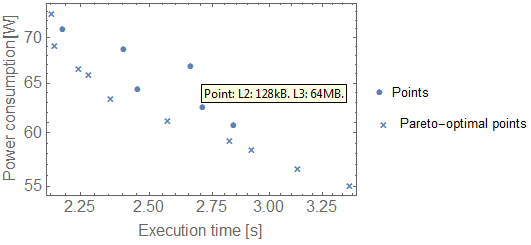
\includegraphics[width=0.8\columnwidth]{img/DSEexample.png}
 \caption{Example DSE Pareto plot.}
 \label{fig:300:dseresult}
\end{figure}

Execution of the design-space exploration can take some time as McPAT is slow to execute. Furthermore, during the design-space exploration Mathematica keeps refreshing the GUI elements in the main notebook regularly, slowing down the process. One way to somewhat speed up the design-space exploration is, after executing the main notebook (ExaBoundsLite.nb) once, to remove the output cells of that notebook. Go to ExaBoundsLite.nb, and select in the \emph{Cell} menu \emph{Delete All Output}. This removes all GUI elements (and they subsequently cannot be used anymore), but IBM ExaBounds stays live in the kernel.

\subsection{Network and full-system design-space exploration}
First we provide an example of a design-space exploration study across different network configurations. The performance metric is the communication time. We assume that the user has an extrapolated profile for an application with one single cluster of MPI processes and a \textit{uniform} communication pattern, such as Graph 500.

The user defines the network architecture properties and the mapping of MPI processes to nodes. 
\begin{mma}
	\In |ExaBoundsState = SetKeyValue[ExaBoundsState|, \linebreak \mathtt{"}|networkConfiguration|\mathtt{"}, \mathtt{"}|fat-tree-3L|\mathtt{"}]; \\
	\In	|ExaBoundsState = SetKeyValue[ExaBoundsState|, \linebreak \mathtt{"}|mappingDescription|\mathtt{"}, <\mid \mathtt{"}|type|\mathtt{"} \rightarrow \mathtt{"}|linear|\mathtt{"} \mid>]; \\
	\In	|ExaBoundsState = SetKeyValue[ExaBoundsState|, \linebreak \mathtt{"}|nodeStackLatency|\mathtt{"}, 0.0000009]; 				\\
	\In	|ExaBoundsState = SetKeyValue[ExaBoundsState|, \linebreak \mathtt{"}|switchLatency|\mathtt{"}, 0.0000007]; 					\\
	\In	|ExaBoundsState = SetKeyValue[ExaBoundsState|, \linebreak \mathtt{"}|switchSwitchBandwidth|\mathtt{"}, 5*1024*1024*1024]; 	\\
	\In	|ExaBoundsState = SetKeyValue[ExaBoundsState|, \linebreak \mathtt{"}|nodeSwitchBandwidth|\mathtt{"}, 5*1024*1024*1024];  	\\
	\In	|ExaBoundsState = SetKeyValue[ExaBoundsState|, \linebreak \mathtt{"}|nodeSwitchLinkLatency|\mathtt{"}, 0.0000000025];  		\\
	\In	|ExaBoundsState = SetKeyValue[ExaBoundsState|, \linebreak \mathtt{"}|switch1Switch2LinkLatency|\mathtt{"}, 0.000000012]; \\
\end{mma}

The user also defines the variations of network architectures to be analyzed. Let's assume that the user analyzes multiple network scenarios of fat-tree-3L topologies for an application with 262144 MPI processes. IBM ExaBounds currently supports assigning one MPI process per node (single-threaded process) and the number of nodes needs to be equal to the number of MPI processes, meaning that the system is fully populated. For a fat-tree-3L, the number of nodes is equal to m1$\cdot$m2$\cdot$m3 which, in this example, should be 262144.
\begin{mma}	
	\In |w0 = \{1, 1, 1, 1\}|; 			\\
	\In	|w1 = \{64, 16, 128, 32\}|; 	\\
	\In	|w2 = \{64, 16, 64, 32\}|; 		\\
	\In	|m1 = \{64, 64, 128, 256\}|; 	\\
	\In	|m2 = \{64, 64, 32, 32\}|; 		\\
	\In	|m3 = \{64, 64, 64, 32\}|; 		\\
	\In |ft3LConfs = Transpose[\{w0, w1, w2, m1, m2, m3\}]|; \\
\end{mma}

For each of the four network scenarios defined above, the user can retrieve the communication time as follows. 
\begin{mma}	
	\In |Do|[\linebreak
		|swProfile = SetKeyValue[swProfile, "topologyDescription"|, \linebreak <\mid \mathtt{"}w0\mathtt{"} \rightarrow |conf[[1]]|, \mathtt{"}w1\mathtt{"} \rightarrow |conf[[2]]|, \mathtt{"}w2\mathtt{"} \rightarrow |conf[[3]]|, \linebreak \mathtt{"}m1\mathtt{"} \rightarrow |conf[[4]]|, \mathtt{"}m2\mathtt{"} \rightarrow |conf[[5]]|, \mathtt{"}m3\mathtt{"} \rightarrow |conf[[6]]| \mid>]; \\
	\In |commTime = GetCommunicationTime[ExaBoundsState, swProfile]|; \\
	\quad , \{conf, ft3LConfs\} ];
\end{mma}

The example above is a simple design-space exploration across the parameters that describe the network topology (in the case of fat-tree-3L, these parameters are w0, w1, w2, m0, m1 and m2). The user can extend this study with more hardware parameters such as latencies or bandwidths.

\vspace{0.5cm}
\begin{minipage}[t]{0.05\textwidth}
	~\\
	\Huge !
\end{minipage}
\begin{minipage}[t]{0.94\textwidth}
	For the network models, IBM ExaBounds currently assumes that all links between switches have the same latency and the same bandwidth. It can be however easily extended to support multiple latencies and bandwidths. Moreover, if the user gets a \textit{missingModel} warning, the user should double-check the name of the topology and the name of the communication pattern. If the topology name or communication pattern is not recognized, IBM ExaBounds does not exit, but prints a warning (Missing model for \textit{topology}: "average link latency", "average number of links", "effective bandwidth").	Thus, the user should always check the warnings.\\
\end{minipage}

Next, to estimate the power consumption of a full system (processors and network), the user must first calculate the processor time (compute, \textit{compTime}) and the network time (communication, \textit{commTime}). In this example, there is only one class of processes, thus we calculate the compute and communication times once (per hardware architecture) and add them to estimate the execution time of the MPI application. This model is reasonable for HPC applications which are typically programmed in a way that minimizes the waiting times and the data dependencies between processes.  If there are multiple classes (clusters) of processes, the user should 1. calculate the compute and communication times per cluster, 2. add them to estimate the time of the process representative of the cluster and 3. estimate the execution time of the MPI application by calculating the maximum time across clusters. This is one possible model to predict application time performance. The user is however free to use any other model for estimating the application time, starting from the IBM ExaBounds processor and network estimates per process or cluster.

In the following we show how the user can estimate the power consumption of the full system (an application with one cluster of MPI processes).
\begin{mma}
	\In |procs = m1*m2*m3|; \\
	\In |appTime = compTime + commTime|; \\
	
	\In	|compPower = Poweri[SocketLayer[], ExaBoundsState, swProfile, False]|; \\
	\In |compPowerStatic = powerProcMem[[1]]|; \\
	\In |compDynamicPower = powerProcMem[[2]]|; \\
	\In |compStaticEnergy = procs*compPowerStatic*appTime|; \\
	\In |compDynamicEnergy = procs*compPowerDynamic*compTime|; \\
	
	\In |commDynamicEnergy = | \linebreak |procs*GetNetworkDynamicEnergy[ExaBoundsState, swProfile]|; \\
	\In |commStaticEnergy = | \linebreak |GetNetworkStaticEnergy[ExaBoundsState, swProfile, appTime]|; \\
	
	\In |systemPower = (compStaticEnergy + compDynamicEnergy +| \linebreak | commStaticEnergy + commDynamicEnergy)/appTime| \\
\end{mma}

The design-space exploration presented at the beginning of this section could be easily extended with the power analysis above so that the user can perform a complete power-performance trade-off analysis. 


\section{Contributors}
\begin{itemize}
  \item Rik Jongerius
  \item Giovanni Mariani
  \item Andreea Anghel
  \item Gero Dittmann
  \item Sandeep Poddar
  \item Phillip Stanley-Marbell
\end{itemize}

\section{Acknowledgement}
This work was conducted in the context of the joint ASTRON and IBM DOME
project and was funded by the Dutch Ministry of Economische Zaken, and the
Province of Drenthe.

\appendix

\section{IBM ExaBounds API}

This appendix describes the most commonly used functions in the ExaBounds API for design-space explorations.

\newcommand*{\call}[2]{\par\noindent\textbf{#1:}\\#2\vspace{5pt}}
\newcommand*{\package}[1]{\vspace{10pt}\par\noindent Package~\textsc{#1}:\vspace{10pt}}

\package{ExaBoundsGeneric}

\call{GetKeyValue[keyValueList\_, key\_]}{Get the value of key \textsc{key} from key-value list \textsc{keyValueList}.}
\call{SetKeyValue[keyValueList\_, key\_, value\_]}{Update the key \textsc{key} in \textsc{keyValueList} with value \textsc{value} and return the updated key-value list.}
\call{MergeKeyValueList[baseList\_, UpdateKeyValuePairs\_]}{Update the \textsc{baseList} key-value pairs with the key-value pairs in \textsc{UpdateKeyValuePairs}, returns the resulting key-value list. All keys in \textsc{UpdatekeyValuePairs} have to be present already in \textsc{baseList}.}
\call{GetAlgorithmName[algInfo\_, index\_]}{Get the name of algorithm with index \textsc{Index} from the \textsc{ExaBoundsAlgInfo} structure. Pass \textsc{ExaBoundsAlgInfo} as the first argument.}
\call{GetAlgorithmKeyValueList[algInfo\_, algoIndex\_,scalingParameters\_, dataProfileId\_,threadId\_] or GetAlgorithmKeyValueList[algInfo\_, sel\_List]}{Retrieve algorithm properties as a key-values list from the \textsc{ExaBoundsAlgInfo} structure. The algorithm is identified as a 4-tuple describing the index, scaling parameters, data profile and thread id, either as individual arguments or as a list.}
\call{SetAlgorithmKeyValue[algInfo\_, sel\_List, key\_, value\_]}{Update a property \textsc{key} of a specific algorithm (identified with a 4-tuple in \textsc{sel}) with \textsc{value} in the \textsc{ExaBoundsAlgInfo} structure. The function is HoldFirst, and does not return anything.}

\textit{The following functions can be used to determine the 4-tuple of algorithm name, scaling configuration, data profile, and thread for applications loaded in the \textsc{ExaBoundsAlgInfo} structure:}\newline

\call{GetScalingParameters[algDataAssociation\_]}{Get the scaling parameters that where used to describe the scale of the algorithm. \textsc{algDataAssociation} is an Association with data for one application, identified as \textsc{ExaBoundsAlgInfo["algorithm name"]}.}
\call{GetScalingConfigurations[algDataAssociation\_]}{Get all scaling configurations that where profiled.}
\call{GetScalingConfigurationsHaving[algDataAssociation\_,partialScalingConfiguration\_]}{Get all scaling configurations that have certain scaling parameters. The scaing configuration is given as an Association.}
\call{GetDataProfileCount[algInfo\_, alg\_, scaling\_]}{Get the number of data profiles from an application in \textsc{ExaBoundsAlgInfo} with name \textsc{alg} and scaling properties \textsc{scaling}.}
\call{GetThreads[algInfo\_, alg\_, scaling\_, profile\_]}{Get the thread identifiers for an application in \textsc{ExaBoundsAlgInfo} with name \textsc{alg}, scaling properties \textsc{scaling} and data profile \textsc{profile}.} 

\package{AlgorithmProperties}

\call{AddAlgorithm[algInfoStructure\_, jsonfile\_]}{Load a IBM Platform-Independent Software Analysis file into \textsc{ExaBoundsAlgInfo} from file \textsc{jsonfile}.}
\call{AppendAlgorithmAnalysis[algInfoStructure\_, newAlgoAnalysis\_}{Append the application profiles in \textsc{newAlgoAnalysis} to \textsc{ExaBoundsAlgInfo}. Used to append algorithms in IBM Exascale Extrapolator *.m-files}

\package{VectorSizeConvert}

\call{GetAlgorithmVectorProperties[archProperties\_, algProperties\_]}{Convert the application properties in \textsc{algProperties} to the vector size in the architecture described by \textsc{archProperties} and return the result. Set the architected vector width to zero for purely scalar instructions.}

\package{PreDefinedMachineConfigs}

\call{LoadArchJSON[file\_]}{Load a processor architecture from \textsc{file}.}
\call{predefinedConfigID2Name}{Replacement list with all available processor architectures and human-readable name.}
\call{predefinedconfig[ configname\_ ]}{Retrieve an architecture named \textsc{configname} (name matching id in \textsc{predefinedConfigID2Name}. Always update \textsc{ExaBoundsState} using \textsc{MergeKeyValueList}.}

\package{PreDefinedNetworkConfigs}

\call{LoadNetworkJSON[file\_]}{Load a network architecture from \textsc{file}.}
\call{predefinedConfigID2NameNetwork}{Replacement list with all available network architectures and human-readable name.}
\call{GetNetworkConfig[ configname\_ ]}{Retrieve a network architecture named \textsc{configname} (name matching id in \textsc{predefinedConfigID2NameNetwork}. Always update \textsc{ExaBoundsState} using \textsc{MergeKeyValueList}.}

\package{PreDefinedMemorySpec}

\call{LoadMemJSON[file\_]}{Load a memory architecture from \textsc{file}.}
\call{predefinedConfigID2NameMem}{Replacement list with all available memory architectures and human-readable name.}
\call{predefinedconfigMem[ configname\_ ]}{Retrieve a memory architecture named \textsc{configname} (name matching id in \textsc{predefinedConfigID2NameNetwork}. Note that the memory architecture name is stored in \textsc{ExaBoundsState} in key \textit{DRAMType}, these properties are not merged into \textsc{ExaBoundsState}.}

\package{CPUPerformanceModels}

\call{CacheHitrate[cacheLevel\_, archProperties\_, algProperties\_]}{Get the hit rate on cache level \textsc{cacheLevel} for application \textsc{algProperties} running on architecture \textsc{archProperties}. The cache levels are listed in Table~\ref{tbl:300:levels} and can be \textsc{MemoryL1Cache[]}, \textsc{MemoryL2Cache[]}, or \textsc{MemoryL3Cache[]}.}
\call{CacheMissrate[cacheLevel\_, archProperties\_, algProperties\_]}{Get the miss rate on cache level \textsc{cacheLevel} for application \textsc{algProperties} running on architecture \textsc{archProperties}.}
\call{AchievedFLOPSi[i\_, archProperties\_, algProperties\_]}{Get the achieved performance at layer \textsc{i} for application \textsc{algProperties} running on architecture \textsc{archProperties}. The layers are listed in Table~\ref{tbl:300:levels} and range from \textsc{CoreLayer[]} to \textsc{SystemLayer[]}.}
\call{BappiDmo[i\_, archProperties\_, algProperties\_]}{Get the achieved memory bandwidth at layer \textsc{i} for application \textsc{algProperties} running on architecture \textsc{archProperties}.}
\call{d0[archProperties\_, algProperties\_]}{Get the performance in cycles per instruction for application \textsc{algProperties} running on architecture \textsc{archProperties}.}
\call{ExecutionCycles[archProperties\_, algProperties\_]}{Get the execution time in clock cycles for application \textsc{algProperties} running on architecture \textsc{archProperties}.}
\call{ExecutionSeconds[archProperties\_, algProperties\_]}{Get the execution time in seconds for application \textsc{algProperties} running on architecture \textsc{archProperties}.}
\call{ClearCPUPerformanceModelsCache[]}{Clear all cached results from the performance models.}

\package{CommunicationPerformanceModels}

\call{GetAverageNetworkLinkLatency[archProperties\_,algProperties\_,tag\_]}{Returns the average number of links (if tag is 1) or the average link latency (if the tag is 0) that an inter-process communication (MPI) message will incur while traversing the network described in \textsc{archProperties} for the communication pattern in \textsc{algProperties}, when the mapping of MPI processes to end nodes is linear and according to the \textit{mappingDescription} parameter in \textsc{archProperties} and the routing is shortest-path with optimal routing when multiple equal-hop routes are available. Default value is 0 (if  the topology or the pattern is not supported). }

\call{UniformAverageNetworkLinkLatency[archProperties\_,tag\_]}{Returns the average number of links (if tag is 1) or the average link latency (if the tag is 0) that an inter-process communication (MPI) message will incur while traversing the network described in \textsc{archProperties} when the communication pattern is uniform, the mapping of MPI processes to end nodes is linear and the routing is shortest-path with optimal routing when multiple equal-hop routes are available. Default value is 0 (if  the topology or the mapping is not supported).}

\call{NNE2DAverageNetworkLinkLatency[archProperties\_,tag\_,D1\_,D2\_]}{Returns the average number of links (if tag is 1) or the average link latency (if the tag is 0) that an inter-process communication (MPI) message will incur while traversing the network described in \textsc{archProperties} when the communication pattern is 2-dimension nearest-neighbor (the 2-dimension application-domain being defined as D1$\cdot$D2), the mapping of MPI processes to end nodes is linear according to the \textit{mappingDescription} parameter in \textsc{archProperties} and the routing is shortest-path with optimal routing when multiple equal-hop routes are available. Default value is 0 (if  the topology or the mapping is not supported).}

\call{ShiftAverageNetworkLinkLatency[archProperties\_,tag\_,shiftValue\_]}{Returns the average number of links (if tag is 1) or the average link latency (if the tag is 0) that an inter-process communication message (MPI) will incur while traversing the network described in \textsc{archProperties} when the communication pattern is shift (the shift value being "shiftValue"), the mapping of MPI processes to end nodes is linear and the routing is shortest-path with optimal routing when multiple equal-hop routes are available. Default value is 0 (if  the topology or the mapping is not supported).}


\call{NodeEffectiveBandwidth[archProperties\_,algProperties\_]}{Returns the node effective TX bandwidth for the network described in \textsc{archProperties} and the communication pattern in \textsc{algProperties}, for when the mapping of MPI processes to end nodes is linear according to the \textit{mappingDescription} parameter in \textsc{archProperties} and the routing is shortest-path with optimal routing when multiple equal-hop routes are available. Default value is the value of the \textit{switchSwitchBandwidth} parameter (if the topology is not supported).}

\call{UniformNodeEffectiveBandwidth[archProperties\_]}{Returns the node effective bandwidth for the network described in \textsc{archProperties} when the communication pattern is uniform, the mapping of MPI processes to end nodes is linear and the routing is shortest-path with optimal routing when multiple equal-hop routes are available. Default value is the value of the \textit{switchSwitchBandwidth} parameter (if the topology is not supported).}

\call{NNE2DNodeEffectiveBandwidth[archProperties\_,D1\_,D2\_]}{Returns the node effective bandwidth for the network described in \textsc{archProperties} when the communication pattern is 2-dimension nearest-neighbor (the 2-dimension application-domain being defined as D1$\cdot$D2), the mapping of MPI processes to end nodes is linear and according to the \textit{mappingDescription} parameter in \textsc{archProperties} and the routing is shortest-path with optimal routing when multiple equal-hop routes are available. Default value is the value of the \textit{switchSwitchBandwidth} parameter (if the topology is not supported).}

\call{ShiftNodeEffectiveBandwidth[archProperties\_,shiftValue\_]}{Returns the node effective bandwidth for the network described in \textsc{archProperties} when the communication pattern is shift (the shift value being \textit{shiftValue}), the mapping of MPI processes to end nodes is linear and the routing is shortest-path with optimal routing when multiple equal-hop routes are available. Default value is the value of the \textit{switchSwitchBandwidth} parameter (if the topology is not supported).}


\call{GetCommunicationTime[archProperties\_,algProperties\_]}{Returns the communication time for the software profile in \textsc{algProperties} and the network hardware description in \textsc{archProperties}. Important note: this is not necessarily the communication time of the application, but the communication time per class/cluster of processes (if \textsc{algProperties} was extracted from an IBM Exascale Extrapolator file) or per MPI process (if \textsc{algProperties} was extracted from a IBM Platform-Independent Software Analysis file with multiple process profiles).}


\package{CommunicationPowerModels}

\call{GetNumberElectricalLinks[archProperties\_,algProperties\_,level\_]}{Returns the average number of electrical links that an inter-process communication (MPI) message traverses through the network. If level is 1, then only the end nodes connected to their switches use electrical links, thus the function returns 2. If level is 2, then all links in the network will be electrical and the function returns the average number of links traversed by an inter-process communication (MPI) message, which is the return value of averageNetworkLinkLatency[1, algProperties\_,archProperties\_]. The return value is either 2 (when only the links connecting the end nodes to the switches are electrical), or the return value of the GetAverageNetworkLinkLatency[archProperties\_,algProperties\_,1] function call (when all links are electrical).}

\call{GetNumberOpticalLinks[archProperties\_,algProperties\_,level\_]}{Returns the average number of optical links that an inter-process communication (MPI) message traverses through the network. If level is 1, then all links except the end nodes connected to their switches use optical links, thus the function returns the difference between the average number of traversed links and the average number of traversed electrical links. If level is 2, then all links in the network will be electrical and the function returns 0. The return value is either GetAverageNetworkLinkLatency[archProperties\_,algProperties\_,1]-2 (when all except the links connecting the end nodes to the switches are optical), or 0 (when no links are optical).}

\call{GetNetworkDynamicEnergy[archProperties\_,algProperties\_]}{Returns the dynamic energy per class/cluster of processes (if \textsc{algProperties} was extracted from an IBM Exascale Extrapolator file) or per process (if \textsc{algProperties} was extracted from a IBM Platform-Independent Software Analysis file with multiple process profiles).}

\call{GetTotalNumberSwitches[archProperties\_]}{Returns the total number of switches in the network described in \textsc{archProperties}. Default value is 1 (if the topology is not supported).}

\call{GetNetworkStaticEnergy[archProperties\_,algProperties\_,appTime\_]}{Returns the static power of the network described in \textsc{archProperties}, when running the application in \textsc{algProperties} for a total duration of time of \textsc{appTime}, comprising both compute and communication time.}


\package{CPUMultithreadedModels}

All multithreaded model functions have the same function prototype as their respective single-core versions with two optional arguments: the first argument \textsc{thread} and the last argument \textsc{homogeneousThreads}. If thread is specified, the function returns the value for the specified thread. If thread is not specified, a list is returned with a value for each thread. 
The last optional argument is used to specify the workload. The workload can be specified as:
\begin{itemize}
 \item a single profile in \textsc{algProperties}, with \textsc{homogeneousThreads} unspecified (or set to 1) for a single-threaded workload (only one core used), e.g. \textsc{MCdo[architecture, profile1]}.
 \item a single profile in \textsc{algProperties}, with \textsc{homogeneousThreads} set to a value \textit{N} for a workload with \textit{N} identical threads (when \textit{N} is larger than the core count, the number of threads will equal the number of cores), e.g. \textsc{MCdo[architecture, profile1, 14]} for 14 threads.
 \item a replacement list of profiles in \textsc{algProperties}. Specify which profile runs on which core, e.g. \textsc{MCdo[architecture, \{1 $\rightarrow$ profile1, 4 $\rightarrow$ profile2\}]}.
\end{itemize}

\call{MCd0[archProperties\_, algProperties\_, homogeneousThreads\_]}{Multi-core version of \textsc{d0}, retrieve performance in cycles per instruction for all threads specified by \textsc{algProperties} and \textsc{homogeneousThreads} as specified above.}
\call{MCd0[thread\_, archProperties\_, algProperties\_, homogeneousThreads\_]}{Multi-core version of \textsc{d0}, retrieve performance in cycles per instruction for \textsc{thread}.}
\call{MCExecutionSeconds[thread\_, archProperties\_, algProperties\_, homogeneousThreads\_]}{Multi-core version of \textsc{ExecutionSeconds}.}
\call{MCExecutionCycles[thread\_, archProperties\_, algProperties\_, homogeneousThreads\_]}{Multi-core version of \textsc{ExecutionCycles}.}
\call{MCCacheMissrate[thread\_, level\_, archProperties\_, algProperties\_, homogeneousThreads\_]}{Multi-core version of \textsc{CacheMissrate}.}
\call{MCBappiDmo[thread\_, level\_, archProperties\_, algProperties\_, homogeneousThreads\_]}{Multi-core version of \textsc{BappiDmo}.}
\call{MCAchievedFLOPSi[thread\_, level\_, archProperties\_, algProperties\_, homogeneousThreads\_]}{Multi-core version of \textsc{AchievedFLOPSi}.}

\call{MCGetKeyValue[algProperties\_, key\_]}{Multi-core version of \textsc{GetKeyValue}. This function returns per-thread values for a given key.}

\package{CPUPowerModels}

The workload for the power models can be specified in a similar way as for the multi-threaded performance models in \textsc{CPUMultithreadedModels}.

\call{Poweri[i\_, archProperties\_, algProperties\_, homogeneousThreads\_]}{Get the system power consumption at layer \textsc{i}.}
\call{PoweriMemory[i\_, archProperties\_, algProperties\_, homogeneousThreads\_]}{Get the memory power consumption at layer \textsc{i}.}
\call{AreaProcessor[archProperties\_, algProperties\_, homogeneousThreads\_]}{Get the total chip area at layer \textsc{i} (McPAT results).}
\call{ClearCPUPowerModelsCache[]}{Clear all cached results from the power models.}
\call{DRAMmodel}{Set the DRAM model, set to either $\mathtt{"}$MeSAP$\mathtt{"}$ or $\mathtt{"}$CACTI$\mathtt{"}$.}

\package{DSEVisualization}

\call{ParetoPlot[data\_List, tooltip\_List]}{Displays Pareto plot. \textsc{Data} is a list of tuples, where each tuple is a design point. \textsc{Tooltip} is an optional argument that can be used to pass a list of human-readable strings describing each design point (both input lists should have the same length). This string is displayed in the plot if the mouse pointer is hovered over a design point. \textsc{ParetoPlot[]} accepts similar options as the Mathematica function \textsc{ListPlot}. Besides the default options, additional options are: \textsc{PlotType}---select the plot type, valid values are \textsc{ListPlot}, \textsc{ListLogPlot}, \textsc{ListLogLinearPlot}, and \textsc{ListLogLogPlot} (default)---, \textsc{ShowParetoPoints}---separately show Pareto points (default: True)---, \textsc{ParetoPointsMarker}---marker used for the Pareto points (default: cross)---, and \textsc{TooltipPrefix}---string prefix used for all tooltips in \textsc{tooltip} (default: Point).}

\section{Architecture parameters}
\label{app:architecture-parameters}

\newcommand*{\param}[3]{\par \noindent \textbf{#1 [#2]:}~#3}

\subsection {Processor architecture parameters}

\param{year}{-}{Year of introduction.}
\param{Lnode}{nm}{Technology node.}
\param{T}{K}{Operating temperature.}
\param{inorder}{True/False}{Inorder core architecture.}
\param{n0}{-}{Core issue width.}
\param{n0dispatch}{-}{Core dispatch width.}
\param{n0threads}{-}{Number of SMT threads per core.}
\param{n0int}{-}{Number of integer functional units per core.}
\param{n0DPFP}{-}{Number of floating-point functional units per core.}
\param{n0mem}{-}{Number of load/store units per core.}
\param{n0control}{-}{Number of branch units per core.}
\param{n0vectorFU}{-}{Number of vector units per core.}
\param{n0vectorbits}{bit}{Vector width.}
\param{T0intop}{cycles}{Average integer instruction forwarding delay.}
\param{T0intmul}{cycles}{Average integer multiply instruction forwarding delay.}
\param{T0intdiv}{cycles}{Average integer division instruction forwarding delay.}
\param{T0fpop}{cycles}{Average floating-point instruction forwarding delay.}
\param{T0fpmul}{cycles}{Average floating-point multiply instruction forwarding delay.}
\param{T0fpdiv}{cycles}{Average floating-point division instruction forwarding delay.}
\param{T0vectorintop}{cycles}{Average vector integer instruction forwarding delay.}
\param{T0vectorintmul}{cycles}{Average vector integer multiply instruction forwarding delay.}
\param{T0vectorintdiv}{cycles}{Average vector integer division instruction forwarding delay.}
\param{T0vectorfpop}{cycles}{Average vector floating-point instruction forwarding delay.}
\param{T0vectorfpmul}{cycles}{Average vector floating-point multiply instruction forwarding delay.}
\param{T0vectorfpdiv}{cycles}{Average vector floating-point division instruction forwarding delay.}
\param{n0Bits}{bit}{Core data path width.}
\param{n1}{-}{Number of cores per die.}
\param{n2}{-}{Number of dies per socket.}
\param{n3}{-}{Number of sockets per card.}
\param{n4}{-}{Number of cards per rack unit.}
\param{n5}{-}{Number of rack units per rack.}
\param{n6}{-}{Number of racks per aisle.}
\param{n7}{-}{Number of aisles per system.}
\param{M0L1}{byte}{Private L1 cache size per core.}
\param{L1dagran}{byte}{L1 data cache granularity (cache line size).}
\param{L1dassoc}{-}{L1 data cache associativity.}
\param{L1iagran}{byte}{L1 instruction cache granularity (cache line size).}
\param{L1iassoc}{-}{L1 instruction cache associativity.}
\param{M0L2}{byte}{Private L2 cache size per core.}
\param{L2dagran}{byte}{L2 cache granularity (cache line size).}
\param{L2dassoc}{-}{L2 cache associativity.}
\param{M1}{byte}{Shared L3 cache size per die.}
\param{L3dagran}{byte}{Shared L3 cache granularity (cache line size).}
\param{L3dassoc}{-}{L3 cache associativity.}
\param{M2}{byte}{DRAM memory per socket.}
\param{nDIMMs}{-}{Number of memory DIMMs per socket.}
\param{nRanksPerDIMM}{-}{Number of ranks per memory DIMM}
\param{DRAMType}{-}{Memory architecture (string with name of memory architecture used).}
\param{T0L1latency}{cycles}{L1 cache access latency.}
\param{T0L2latency}{cycles}{L2 cache access latency (including L1 latency).}
\param{T0L3latency}{cycles}{L3 cache access latency (including L1 and L2 latency).}
\param{T0DRAMlatency}{cycles}{DRAM access latency (including cache latency).}
\param{B0Dmo}{byte/s}{Core to L1/L2 cache bandwidth.}
\param{B1Dmo}{byte/s}{L2 cache to L3 cache bandwidth.}
\param{B2Dmo}{byte/s}{L3 cache to DRAM bandwidth.}
\param{f0}{Hz}{Core clock speed.}
\param{f1}{Hz}{Processor bus clock speed.}
\param{n0pipe}{-}{Core pipeline depth.}
\param{n0frontpipe}{-}{Core front-end pipeline depth.}
\param{n0ROB}{-}{Core reorder buffer size.}
\param{n0IQ}{-}{Core issue queue size.}
\param{n0MSHR}{-}{Core miss-status holding register count.}
\param{V0}{V}{Core voltage.}

\subsection{Memory architecture parameters}

\param{MemoryId}{-}{Name of memory configuration.}
\param{MemoryType}{-}{Memory type (DDR3/4).}
\param{MemoryRankSize}{Gb}{Size of a memory rank.}
\param{DevicesPerRank}{-}{Number of memory devices (chips) per rank.}
\param{DeviceChipSize}{MB}{Size of memory device.}
\param{DataWidth}{bit}{Data bus width of a memory device.}
\param{DataRate}{1/cycle}{Single or dual data rate.}
\param{BurstLength}{-}{Maximum supported burst length.}
\param{ClkMHz}{Hz}{Memory bus clock frequency.}
\param{REFI}{cycles}{Refresh interval. DRAM is required to go through a refresh cycle once in this refresh interval.}
\param{RFC}{cycles}{Refresh cycle. The time between the start of a refresh and activation commands.}
\param{RAS}{cycles}{Row access strobe. Minimum time interval between a row activation and precharge command for data restoration.}
\param{RP}{cycles}{Row precharge. Time to close an active row.}
\param{idd0}{mA}{Operating one bank Active-Precharge current. The command consists of one ACT and one PRE command to one bank in sequence. All other banks are in precharged state.}
\param{idd2n}{mA}{Precharge Standby Current. All banks are in precharged state.}
\param{idd3n}{mA}{Active Standby current. One bank is in active state and others are in precharged state.}
\param{idd4r}{mA}{Burst Read Current. Continuous burst reads using RD commands. All banks open.}
\param{idd4w}{mA}{Burst Write Current. Continuous burst writes using WR commands. All banks open.}
\param{idd5b}{mA}{Refresh current. Issued every tRFC cycles.}
\param{vdd}{V}{Operating voltage.}

\subsection{Network architecture parameters}

\hspace{0.5cm} In the following list of parameters that describe the network architecture, "X:Y" means that parameter "Y" is defined as part of the "X" JSON object. The same for "X:Y:Z" which means that "Z" is defined as part of the "Y" JSON object which is a part of the "X" JSON object.\\

\param{id}{-}{Network topology ID. Currently it can be fat-tree-2L, fat-tree-3L, 2DhyperX, full-mesh, torus-1D, torus-2D, torus-3D, torus-5D.}
\param{name}{-}{Network topology name. Currently it can be Fat tree 2L, Fat tree 3L, 2DhyperX, Full-mesh, Torus-1D, Torus-2D, Torus-3D, Torus-5D.} \\

ExaBounds currently provides network models for the following topologies:
\begin{itemize}
	\item uniform communication pattern: full-mesh, fat-tree-2L, fat-tree-3L, 2D Hyper-X, multi-dimensional tori.
	\item shift communication pattern: full-mesh, fat-tree-2L, fat-tree-3L.
	\item 2-dimension nearest-neighbor communication pattern: full-mesh, fat-tree-2L, fat-tree-3L, 2D Hyper-X.
\end{itemize}

\param{config:topologyDescription}{-}{A list of network topology parameters that describe the network configuration. 
This object includes multiple parameters depending on the topology id (see below).} \\

Topology description parameters per topology id:
\begin{itemize}
	\item full-mesh: "a" (number of switches in the network) and "p" (number of end nodes connected to a switch). 
	%\item dragonfly: "a" (number of switches in a dragonfly group), "p" (number of end nodes connected to a switch),"h" (number of external links per switch that connects to switches in other groups). 
	\item fat-tree-2L: "w0" (the number of up-links in level-1 switches), "w1" (the number of up-links in level-2 switches), "m1" (the number of down-links in level-1 switches) and "m2" (the number of down-links in level-2 switches).
	\item fat-tree-3L: "w0" (the number of up-links in level-1 switches), "w1" (the number of up-links in level-2 switches), "w2" (the number of up-links in level-3 switches),"m1" (the number of down-links in level-1 switches), "m2" (the number of down-links in level-2 switches) and "m3" (the number of down-links in level-3 switches). 
	\item 2DhyperX: "p" (the number of end nodes connected to a switch), "d1" (the number of switches in the X dimension) and "d2" (the number of switches in the Y dimension). 
	\item torus-Nd: "p" (the number of end nodes connected to a switch), "d1" (the number of switches in the 1st dimension) ... "dN" (the number of switches in the N-th dimension), where N$\geq$1. \\
\end{itemize} 

\param{config:nodeStackLatency}{second}{End node MPI stack latency.}
\param{config:switchLatency}{second}{Switch internal latency.}
\param{config:nodeSwitchLinkLatency}{second}{Link latency between the end node and the switch to which the end node is connected.}
\param{config:switch1Switch2LinkLatency}{second}{Link latency between two directly connected switches. For a fat-tree-2L and fat-tree-3L topologies, this is the link between a level-1 switch and a level-2 switch. For a full-mesh, this is the link between two directly connected switches. For a 2D Hyper-X, this is the link between two directly connected switches. Similar for multi-dimension tori topologies.}
\param{config:switch2Switch3LinkLatency}{second}{[Valid only for fat-tree 3L topologies] Link latency between a level-2 switch and a level-3 switch.} \\
%\param{config:intraGroupSwitchSwitchLinkLatency}{second}{[Valid only for dragonfly topologies] Link latency between two directly connected switches both 
%	located in a dragonfly group.}
%\param{config:interGroupSwitchSwitchLinkLatency}{second}{[Valid only for dragonfly topologies] Link latency between two directly connected switches 
%	located in different dragonfly groups.} \\

\param{config:nodeSwitchBandwidth}{byte/s}{Link bandwidth between the end node and the switch to which the end node is connected.}
\param{config:switchSwitchBandwidth}{byte/s}{Link bandwidth between two directly connected switches. Currently supported: all switch-switch links have the same bandwidth.} \\

Currently ExaBounds supports two possible combinations of types (electrical/optical) of links in the network: 1. All links in the network are electrical. 2. The end nodes are connected to their switch via electrical links and all the remainder links connecting switches are all optical. \\

\param{config:nodeSwitchLinkType}{electrical/optical}{Type of link between the end node and the switch to which the end node is connected.}
\param{config:switch1Switch2LinkType}{electrical/optical}{Type of link between two directly connected switches. For a fat-tree-2L and fat-tree-3L topologies, this is the link between a level-1 switch and a level-2 switch. For a full-mesh, this is the link between two directly connected switches. For a 2D Hyper-X, this is the link between two directly connected switches. Similar for multi-dimension tori topologies.}
\param{config:switch2Switch3LinkType}{electrical/optical}{[Valid only for fat-tree 3L topologies] Type of link between a level-2 switch and a level-3 switch.}
%\param{config:intraGroupSwitchSwitchLinkType}{electrical/optical}{[Valid only for dragonfly topologies] Type of link between two directly connected switches 
%	both located in a dragonfly group.}
%\param{config:interGroupSwitchSwitchLinkType}{electrical/optical}{[Valid only for dragonfly topologies] Type of link between two directly connected switches 
%	both located in different dragonfly groups.} \\

\param{config:electricalLinkEnergyPerBit}{pJ}{Energy per bit in electrical links.}
\param{config:opticalLinkEnergyPerBit}{pJ}{Energy per bit in optical links.}
\param{config:switchLogicEnergyPerBit}{pJ}{Energy per bit in the switch.}
\param{config:switchStaticPower}{W}{Static power per switch.} \\

When dealing with applications running on parallel systems, the MPI rank mapping plays an important role for the system performance. 
For the uniform and shift communication patterns, ExaBounds currently provides network performance models only for linear mappings. 
For the 2-dimension nearest-neighbor pattern, we cover more than just linear mappings as follows. \\

ExaBounds models mappings where the application domain (the grid of processes that
determines the 2-dimension nearest-neighbor pattern) is partitioned into equal-sized application sub-domains.
The domain of hardware nodes is assumed to be also partitioned into same-sized hardware sub-domains. 
E.g., for the full-mesh topology, the partitioning of the set of hardware nodes into sub-sets each belonging to the same switch is such a partition.
The size of an application sub-domain should be equal to the size of a hardware sub-domain.
The mappings that ExaBounds covers are those that bijectively map the application sub-domains onto the hardware sub-domains. 
Thus not only must the total number of end nodes in the system match the total
number of application processes, but the processes in an application sub-domain
should also fully populate the compute nodes in a hardware sub-domain.  
Currently, for the 2-dimension nearest-neighbor pattern, ExaBounds provides network performance models only for 
full-mesh, fat-tree 2L, fat-tree 3L and 2D Hyper-X topologies. \\

\param{config:mappingDescription:type}{linear}{Always set to linear. For uniform and shift application communication patterns, only this parameter is required for describing the mapping of MPI processes to end nodes. For the 2-dimension nearest-neighbor pattern, additional parameters should to be defined as follows (see below).} \\

If the 2-dimension nearest-neighbor application domain is of size D1$\cdot$ D2. 
\begin{itemize}
	\item full-mesh: the mapping should be described by a tuple $\{$d11$,$d12$\}$, where d11$\cdot$d12$=$p, d11 divides D1 and d12 divides D2, meaning that the processes of each application sub-domain of size d11$\cdot$d12 is linearly mapped to the end nodes of a switch. 
	\item fat-tree-2L: the mapping should similarly be described by a tuple $\{$d11$,$d12$\}$, where d11$\cdot$d12$=$m1, d11 divides D1 and d12 divides D2, meaning that the processes of each application sub-domain of size d11$\cdot$d12 is linearly mapped to the end nodes of a level-1 switch. 
	\item fat-tree-3L: the mapping should be described by a 4 values $\{$d11$,$d12$,$d21$,$d22$\}$, where d21$\cdot$d22$=$m1, d11$\cdot$d12$=$m1$\cdot$m2, d21 divides d11, d22 divides d12, d11 divides D1 and d12 divides D2. In this case, the application domain is divided into sub-domains of size d11$\cdot$d12 and each sub-domain into sub-sub-domains of size d21$\cdot$d22. Each application sub-domain is mapped linearly to the end nodes of a level-2-switch-rooted sub-tree and each application sub-sub-domain is mapped linearly to the end nodes of a level-1 switch of the level-2-switch-rooted sub-tree. 
	\item 2DhyperX: the application sub-domain is represented by a line in the application domain. The hardware sub-domain is represented by all the nodes connected to a set of m $\in\{$1,2, ... d1$\}$ consecutive switches in the X dimension of the network topology. To describe the mapping in the case of 2D Hyper-X topologies the user only has to define the "type" parameter as "linear".
\end{itemize}

\param{config:mappingDescription:d11}{-}{[Valid only for the 2-dimension nearest-neighbor pattern] This parameter needs to be defined for full-mesh, fat-tree-2L and fat-tree-3L topologies.}
\param{config:mappingDescription:d12}{-}{[Valid only for the 2-dimension nearest-neighbor pattern] This parameter needs to be defined for full-mesh, fat-tree-2L and fat-tree-3L topologies.}
\param{config:mappingDescription:d21}{-}{[Valid only for the 2-dimension nearest-neighbor pattern] This parameter needs to be defined fat-tree-3L topologies.}
\param{config:mappingDescription:d22}{-}{[Valid only for the 2-dimension nearest-neighbor pattern] This parameter needs to be defined fat-tree-3L topologies.}


\bibliographystyle{ieeetr}
\bibliography{manual}

\end{document}
